\setcounter{equation}{0}
\par \Def Уравнение вида
\begin{equation}\label{cauchy-zero}
    F(x_1, \ldots, x_n, u, \frac{\partial u}{\partial x_1}, \ldots, \frac{\partial u}{\partial x_n}) = 0,
\end{equation}
\par где $n \geq 2$, $F(x_1, \ldots, x_n, u, p_1, \ldots, p_n)$~--- заданная действительная непрерывно дифференцируемая функция в некоторой области $G$ $(2n + 1)$\,-мерного
пространства с декартовыми прямоугольными координатами $x_1, \ldots, x_n, u, p_1, \ldots, p_n$ и в каждой точке $G$
$$\sum_{i=1}^n \left(\frac{\partial F}{\partial p_i}\right)^2 \neq 0$$
\par называется дифференциальным уравнением в частных
производных первого порядка относительно неизвестной функции $u = u(x_1, \ldots, x_n)$

\par \Def Функция $\varphi(x_1, \ldots, x_n)$, заданная в области $\Omega$ пространства $\mathbb{R}_{(x_1, \ldots, x_n)}^n$ называется решением уравнения (\ref{cauchy-zero}), если:
\begin{enumerate}
    \item $\varphi(x_1, \ldots, x_n)$ - непрерывно дифференцируемая функция в $\Omega$
    \item для всех точек $(x_1, \ldots, x_n)\in \Omega$ точка $(x_1, \ldots, x_n, \varphi(x_1, \ldots, x_n), \frac{\partial \varphi}{\partial x_1}, \ldots, \frac{\partial \varphi}{\partial x_n}) \in G$
    \item $F(x_1, \ldots, x_n, \varphi(x_1, \ldots, x_n), \frac{\partial \varphi}{\partial x_1}, \ldots, \frac{\partial \varphi}{\partial x_n}) \equiv 0, \forall (x_1, \ldots, x_n)\in \Omega$
\end{enumerate}

\par \Def Решение уравнения (\ref{cauchy-zero}) в $(n+1)$-мерном пространстве $\mathbb{R}_{(x_1, \ldots, x_n)}^{n+1}$ задает некоторую гладкую поверхность размерности $n$ (гиперповерхность), которая называется интегральной поверхностью уравнения (\ref{cauchy-zero}).

\par \Def Уравнения вида $$\sum_{j=1}^n a_j(x_1, \ldots, x_n) \frac{\partial u}{\partial x_j} = 0$$
\par называется линейным однородным уравнением в частных производных первого порядка.

\par Пусть $x=(x_1, \ldots, x_n)$, принадлежит $\Omega$ - некоторой области пространства $\mathbb{R}_x^n, n \geqslant 2$. В области $\Omega$ рассмотрим линейное однородное уравнение в
частных производных первого порядка
\begin{equation}\label{cauchy-first}
    \sum_{j=1}^n a_j(x) \frac{\partial u(x)}{\partial x_j}=0,
\end{equation}
\par где $a_j(x)$ - заданные непрерывно дифференцируемые в $\Omega$ функции, $j=1, \ldots, n$, для которых
\begin{equation}\label{cauchy-second}
    \sum_{j=1}^n a_j^2(x) \neq 0, \: \forall x \in \Omega
\end{equation}

\par Если ввести вектор-функцию $a(x)$ с компонентами $a_1(x), \ldots, a_n(x)$, то уравнение (\ref{cauchy-first}) сокращенно можно записать с помощью скалярного произведения в следующем виде:
\begin{equation}\label{cauchy-third}
    (a(x), grad \: u(x))=0
\end{equation}

\par \Def Автономная система 
\begin{equation}\label{cauchy-fourth}
    \dot{x}(t)=a(x)
\end{equation}
\par называется характеристической системой уравнения (\ref{cauchy-first}), а траектории системы (\ref{cauchy-fourth}) называются характеристиками уравнения (\ref{cauchy-first}).

\par \Note Условие (\ref{cauchy-second}) означает, что область $\Omega$ не содержит положений равновесия характеристической системы (\ref{cauchy-fourth})

\par \textbf{Теорема 1.} В некоторой окрестности каждой точки $b \in \Omega$ все решения уравнения (\ref{cauchy-first}) имеют вид 
$$u(x)=F[u_1(x), \ldots, u_{n-1}(x)],$$
\par где $u_j(x)$, $j=1, \ldots, n-1$, - независимые в точке $b$ первые интегралы характеристической системы (\ref{cauchy-fourth}), a $F(\zeta_1, \ldots, \zeta_{n-1})$ — произвольная непрерывно дифференцируемая функция.

\par \Proof По теореме 1 из билета 6.1 все решения уравнения (\ref{cauchy-first}) являются первыми интегралами характеристической системы (\ref{cauchy-fourth}), так как уравнение (\ref{cauchy-first}) равносильно тому, что производная в силу системы (\ref{cauchy-fourth}) $\dot{u}(x)=0$ в области $\Omega$. При условии (\ref{cauchy-second}) из теоремы 3 билета 6.1, в некоторой
окрестности $V \subset \Omega$ точки $b \in \Omega$ существуют $(n-1)$ независимых в точке $b$ первых интегралов $u_1(x), \ldots, u_{n-1}(x)$ системы (\ref{cauchy-fourth}) и любой первый
интеграл (\ref{cauchy-fourth}) имеет вид
$$u(x)=F[u_1(x), \ldots, u_{n-1}(x)],$$
\par где $F(\zeta_1, \ldots, \zeta_{n-1})$ — произвольная непрерывно дифференцируемая функция. \EndProof

\par \Def Функция $u(x)=F[u_1(x), \ldots, u_{n-1}(x)],$ где $F(\zeta_1, \ldots, \zeta_{n-1})$ — произвольная непрерывно дифференцируемая функция своих аргументов, называется общим решением уравнения (\ref{cauchy-first}) в окрестности $V$ точки $b \in \Omega$.

\par \Note Из доказанной теоремы 1 следует, что характеристики являются линиями уровня интегральной поверхности уравнения (\ref{cauchy-first}).

\par Пусть уравнение
$$g(x)=0$$
\par задает в области $\Omega$ гладкую $(n-1)$-мерную поверхность (т. е. гиперповерхность) $\gamma$ ($g(x)$ - непрерывно дифференцируема и $grad \: g(x) \neq 0,\: \forall x \in \Omega$).
Эта поверхность $\gamma$ называется начальной поверхностью. Пусть, кроме того, на поверхности $\gamma$ задана некоторая непрерывно дифференцируемая функция $\varphi(x)$.

\par Зададим начальное условие
\begin{equation}\label{cauchy-sixth}
    u(x)|_{x\in \gamma}=\varphi(x)
\end{equation}
\par Функция $\varphi(x)$ называется начальным значением $u(x)$.

\par \textbf{Задача Коши} для уравнения (\ref{cauchy-first}): Найти такое решение уравнения (\ref{cauchy-first}), которое удовлетворяет начальному условию (\ref{cauchy-sixth}).
\par \textbf{Геометрический смысл:}
\begin{center}
    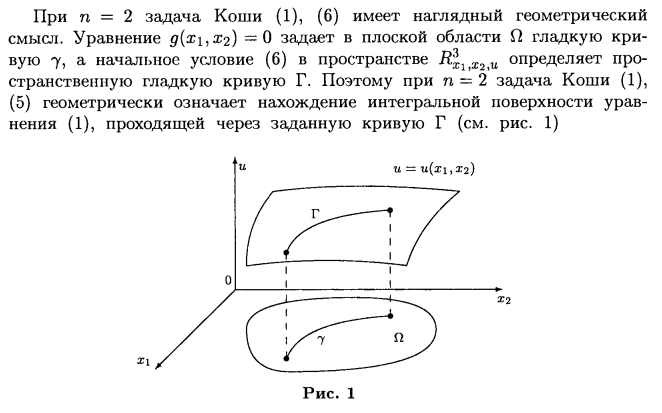
\includegraphics[scale=1.1]{sections/Dima/images/cauchy.png}
\end{center}
\par \Def Всякая точка $M_0 \in \gamma$, для которой
$$\dot{g}(M_0)=(a(M_0), grad \: g(M_0))=0,$$
\par называется характеристической точкой уравнения (\ref{cauchy-first}).

\par \Note Тот факт, что $M_0 \in \gamma$ является характеристической точкой (\ref{cauchy-first}), геометрически означает, что вектор $a(M_0)$ касается поверхности $\gamma$ в точке $M_0$
или, что то же самое, касается характеристик (\ref{cauchy-first}) в точке $M_0$. В частности, положения равновесия характеристической системы (\ref{cauchy-fourth}) и особые точки поверхности $\gamma$ являются характеристическим точками уравнения (\ref{cauchy-first}). Если при $n=2$ кривая $\gamma$ является характеристикой (\ref{cauchy-first}), то каждая точка $\gamma$ является характеристической точкой (\ref{cauchy-first}).

\par \textbf{Теорема 2.} Если $M_0 \in \gamma$ не является характеристической точкой уравнения (\ref{cauchy-first}), то в некоторой окрестности $V \subset \Omega$ точки $M_0$ решение задачи
Коши (\ref{cauchy-first}), (\ref{cauchy-sixth}) существует и единственно.

\par \Proof Так как $M_0$ не характеристическая точка, то $a(M_0) \neq 0$, значит в некоторой окрестности $V$ точки $M_0$ существуют $(n -1)$ независимые в точке $M_0$ первые интегралы $u_l(x), l=1, \ldots, n-1$, характеристической системы (\ref{cauchy-fourth}). По теореме 1 в окрестности $V$ общее
решение (\ref{cauchy-first}) имеет вид
$$u(x)=F[u_1(x), \ldots, u_{n-1}(x)],$$
\par где $F$ — произвольная непрерывно дифференцируемая функция. Покажем, что начальное условие (\ref{cauchy-sixth}) однозначно определяет вид функции $F$. С этой целью в окрестности $V$ рассмотрим систему уравнений
\begin{equation}\label{cauchy-seventh}
    \begin{cases}
      u_l(x)=u_l, l = 1, \ldots, n-1\\
      g(x)=0
    \end{cases}\,.
\end{equation}
\par Покажем, что систему (\ref{cauchy-seventh}) можно однозначно разрешить относительно $x=(x_1, \ldots, x_n)$ в окрестности $V$. Проверим для системы (\ref{cauchy-seventh}) выполнение условий теоремы о системе неявных функций.
\par Все функции в системе (\ref{cauchy-seventh}) непрерывно дифференцируемы в окрестности $V$. Осталось показать, что якобиан
$$\left. \frac{\partial (u_1, \ldots, u_{n-1}, g)}{\partial (x_1, \ldots, x_n)}\right|_{M_0} \neq 0$$
\par Рассуждаем от противного. Пусть якобиан равен нулю. Так как первые $(n-1)$ строк якобиана линейно независимы, то в таком случае последняя его строка линейно зависит от его первых $(n-1)$ строк. Следовательно, найдутся числа $c_l$, $l=1, \ldots, n-1$, одновременно не равные нулю, такие, что
$$\frac{\partial g(M_0)}{\partial x_j}=\sum_{l=1}^{n-1} c_l \frac{\partial u_l(M_0)}{\partial x_j}, \: \forall j = 1, \ldots, n$$
\par Поэтому
$$\dot{g}(M_0)=\sum_{j=1}^n a_j(M_0) \frac{\partial g(M_0)}{\partial x_j}=\sum_{j=1}^n a_j(M_0) \sum_{l=1}^{n-1} c_l \frac{\partial u_l(M_0)}{\partial x_j}=\sum_{l=1}^{n-1} c_l \sum_{j=1}^n a_j(M_0) \frac{\partial u_l(M_0)}{\partial x_j}=\sum_{l=1}^{n-1} c_l \dot{u}_l(M_0)=0$$

\par в силу того, что $u_l(x), l=1, \ldots, n-1$ — первые интегралы (\ref{cauchy-fourth}).

\par С другой стороны, $\dot{g}(M_0) \neq 0$, так как по условию теоремы $M_0 \in \gamma$ не является характеристической точкой (\ref{cauchy-first}). Противоречие. Поэтому в окрестности $V$ выполнены все условия теоремы о неявной функции и система уравнений (\ref{cauchy-seventh}) допускает в окрестности $V$ единственное
непрерывно дифференцируемое решение $x=\omega(u_1, \ldots, u_{n-1})$.

\par Для всех $x \in \gamma \cap V$ функция
$$\varphi(x)=\varphi[\omega(u_1, \ldots, u_{n-1})] \equiv \Phi(u_1, \ldots, u_{n-1})$$
\par является известной непрерывно дифференцируемой функцией $u_1, \ldots, u_{n-1}$. По построению отсюда следует, что
$$u(x)=\Phi[u_1(x), \ldots, u_{n-1}(x)]$$
\par является искомым единственным решением задачи Коши (\ref{cauchy-first}), (\ref{cauchy-sixth}) в окрестности V, так как $u(x)$ — первый интеграл (\ref{cauchy-fourth}) и удовлетворяет начальному условию (\ref{cauchy-sixth}). \EndProof
